% Chapter 2

\chapter{Project 2a: Matrix multiplication} % Main chapter title

\label{Chapter2} % for referencing this chapter elsewhere, use \ref{Chapter2}

\lhead{Chapter 2. \emph{Matrix multiplication}} % this is for the header on each page - perhaps a shortened title

%----------------------------------------------------------------------------------------


\section{Introduction}



\section{Implementations \citep{matrixMultiplication}}


\subsection{Naive}


\subsection{Naive - transposed}


\subsection{Recursive}
The recursive multiplication is implemented as follows:
\begin{verbatim}
   int m = heightA;
  int n = widthA;
  int p = (*matrixB).nCols;
  B = matrixB;
  C = createMatrix(m, p);
  
  recMult(0, 0, 0, 0, m, n, p);
  
  return C;
\end{verbatim}

It makes use of the following recursive method:
\begin{verbatim}
void recMult(int i_A, int j_A, int i_B, int j_B, int m, int n, int p) {
  if (m==1 && n==1 && p==1) { // base case
    int AB = matrixGet(A, i_A, j_A)*matrixGet(B, i_B, j_B);
    matrixAdd(C, i_A, j_B, AB);
  } else if (m >= max(n,p)) { // split rows of A
    recMult(i_A,     j_A,     i_B,     j_B,     m/2,   n,     p    );
    recMult(i_A+m/2, j_A,     i_B,     j_B,     m-m/2, n,     p    );
  } else if (n >= max(m,p)) { // split columns of A and rows of B
    recMult(i_A,     j_A,     i_B,     j_B,     m,     n/2,   p    );
    recMult(i_A,     j_A+n/2, i_B+n/2, j_B,     m,     n-n/2, p    );
  } else if (p >= max(m,n)) { // split columns of B
    recMult(i_A,     j_A,     i_B,     j_B,     m,     n,     p/2  );
    recMult(i_A,     j_A,     i_B,     j_B+p/2, m,     n,     p-p/2);
  }
  return;
}
\end{verbatim}



\subsection{Tiled}



\section{Results and discussion}



\begin{figure}[htbp]
	\centering
		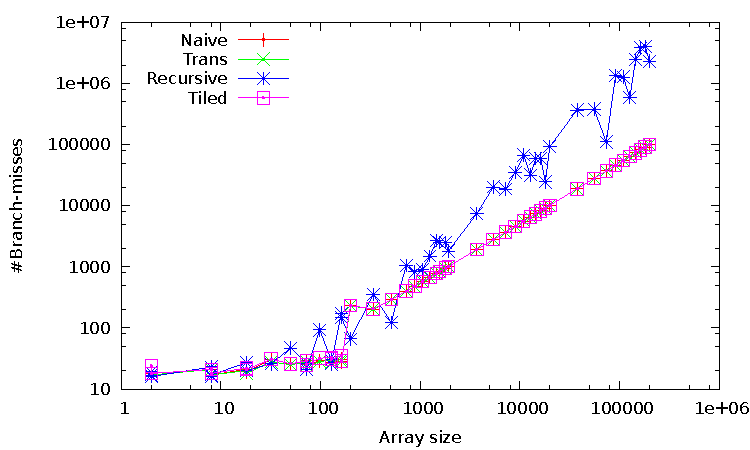
\includegraphics[width=\textwidth]{./Figures/Project2a/Branch_misses.pdf}
		\rule{35em}{0.5pt}
	\caption[Branch misses]{
	Bla bla bla.
	}
	\label{fig:Branch_misses}
\end{figure}


\begin{figure}[htbp]
	\centering
		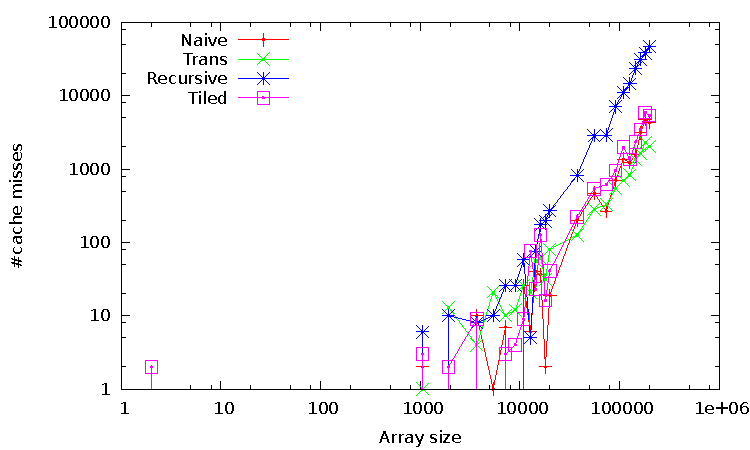
\includegraphics[width=\textwidth]{./Figures/Project2a/Cache_misses.pdf}
		\rule{35em}{0.5pt}
	\caption[Cache misses]{
	Bla bla bla.
	}
	\label{fig:Cache_misses}
\end{figure}



\begin{figure}[htbp]
	\centering
		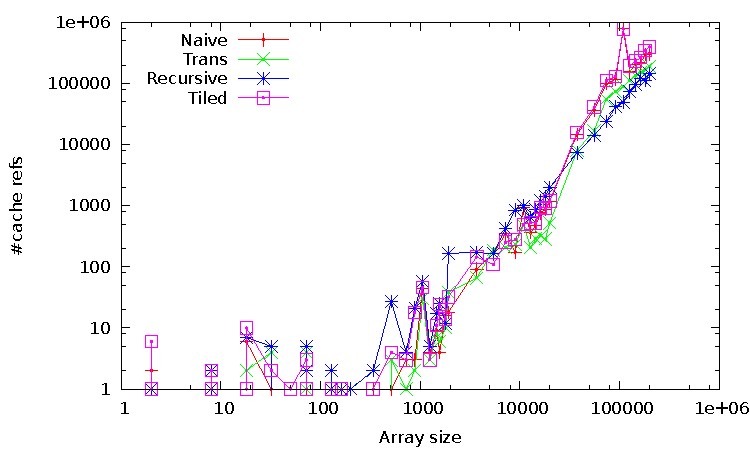
\includegraphics[width=\textwidth]{./Figures/Project2a/Cache_refs.pdf}
		\rule{35em}{0.5pt}
	\caption[Cache refs]{
	Bla bla bla.
	}
	\label{fig:Cache_refs}
\end{figure}



\begin{figure}[htbp]
	\centering
		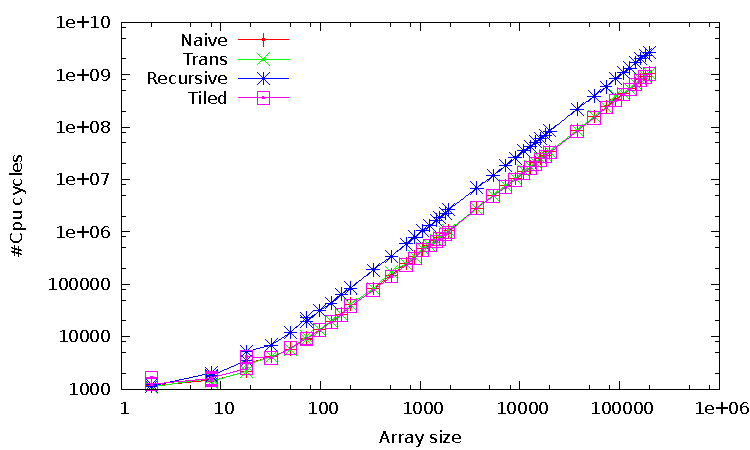
\includegraphics[width=\textwidth]{./Figures/Project2a/Cpu_cycles.pdf}
		\rule{35em}{0.5pt}
	\caption[CPU cycles]{
	Bla bla bla.
	}
	\label{fig:Cpu_cycles}
\end{figure}


\begin{figure}[htbp]
	\centering
		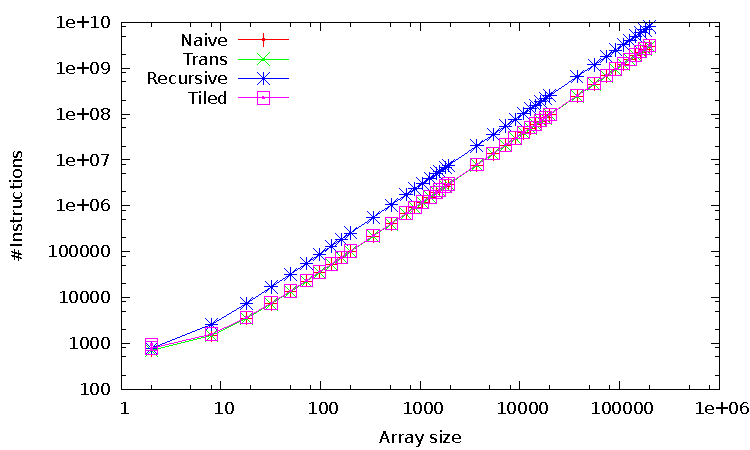
\includegraphics[width=\textwidth]{./Figures/Project2a/Instructions.pdf}
		\rule{35em}{0.5pt}
	\caption[Instructions]{
	Bla bla bla.
	}
	\label{fig:Instructions}
\end{figure}
